%%%%%%%%%%%%%%%%%%%%%%%%%%%%%%%%%%%%%%%%%%%%%%%%%%%%%%%%%%%%%%%%%%%%%%%%%%%%%%%%%%%
% Team: Rainy
% Members: Rain  Dickson  Sareddy
% Relative files:
% Note: Do not compile this file compile Main.tex to get the pdf file instead.
%%%%%%%%%%%%%%%%%%%%%%%%%%%%%%%%%%%%%%%%%%%%%%%%%%%%%%%%%%%%%%%%%%%%%%%%%%%%%%%%%%%
\subsection{Latent Semantic Analysis}
Latent Semantic Analysis is a kind of Corpus-Based similarity anaysis. Corpus-Based similarity is a semantic similarity measure which determines the similarity between the words based on the information gained from corpora. A Corpus is a large collection of texts and it is used for language research. Latent Semantic Analysis(LSA) assumesthat the words with close meaning will mostly occur inthe similar group. A matrix which contains word counts per paragraph was constructed from a  dataset.In order to reduce the number of columns, singular ue decomposition (SVD) is used and it preserves the similarity structure among the rows. The LSA approach is extended by focusing on term vectors instead of the representation of dual document-term and cosine measures between the vectors are expressed based on the semantic relatedness between two texts.
 
\subsection{Metadata Extraction}
Metadata Extractor is the module which can extract metadata in PDF files such as title, subheading, doi, etc. We use python package pyPdf to extract metadata directly and use metadata to do a couple of things. First, we extract titles of articles returning those to the web page as search results. Second, we use metadata extractor to extract subheadings which are treated as the definition of break point to split PDF file i.e. one article will be separated into small pieces based on subheading. The small pieces will convert into .txt files by the .txt converter we built so that we can take .txt files into similarity comparison and get the most relative parts in the article.Third, We extract doi [explain what is doi] which can link to the original article source. 
      \subsection{Extracting Information from Text}
For any given question, it's likely that someone has written the answer down somewhere. The amount of natural language text that is available in electronic form is truly staggering, and is increasing every day. 
However, the complexity of natural language can make it very difficult to access the information in that text. The state of the art in NLP is still a long way from being able to build general-purpose representations of meaning from unrestricted text. 
If we instead focus our efforts on a limited set of questions or "entity relations," such as "where are different facilities located," or "who is employed by what company," we can make significant progress.
\subsection{Similarity Comparison}
	\begin{figure*}[htb]
		\begin{center}
			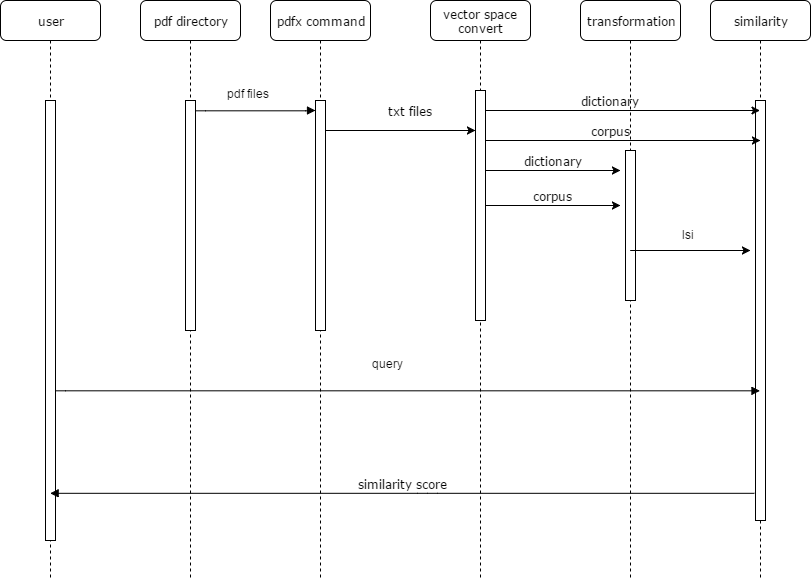
\includegraphics[width=0.8\textwidth]{Rainy_Sequence_diagram}
		\end{center}
		\caption{Sequence diagram of text similarity compare function.\label{Sequence diagram}}
	\end{figure*}
	\newpage